\documentclass[]{book}
\usepackage{lmodern}
\usepackage{amssymb,amsmath}
\usepackage{ifxetex,ifluatex}
\usepackage{fixltx2e} % provides \textsubscript
\ifnum 0\ifxetex 1\fi\ifluatex 1\fi=0 % if pdftex
  \usepackage[T1]{fontenc}
  \usepackage[utf8]{inputenc}
\else % if luatex or xelatex
  \ifxetex
    \usepackage{mathspec}
  \else
    \usepackage{fontspec}
  \fi
  \defaultfontfeatures{Ligatures=TeX,Scale=MatchLowercase}
\fi
% use upquote if available, for straight quotes in verbatim environments
\IfFileExists{upquote.sty}{\usepackage{upquote}}{}
% use microtype if available
\IfFileExists{microtype.sty}{%
\usepackage{microtype}
\UseMicrotypeSet[protrusion]{basicmath} % disable protrusion for tt fonts
}{}
\usepackage[margin=1in]{geometry}
\usepackage{hyperref}
\PassOptionsToPackage{usenames,dvipsnames}{color} % color is loaded by hyperref
\hypersetup{unicode=true,
            pdftitle={Mathematics for Deep Learning and Artificial Intelligence},
            pdfauthor={Christian Ramsey \& Haohan Wang},
            colorlinks=true,
            linkcolor=Maroon,
            citecolor=Blue,
            urlcolor=Blue,
            breaklinks=true}
\urlstyle{same}  % don't use monospace font for urls
\usepackage{natbib}
\bibliographystyle{apalike}
\usepackage{longtable,booktabs}
\usepackage{graphicx,grffile}
\makeatletter
\def\maxwidth{\ifdim\Gin@nat@width>\linewidth\linewidth\else\Gin@nat@width\fi}
\def\maxheight{\ifdim\Gin@nat@height>\textheight\textheight\else\Gin@nat@height\fi}
\makeatother
% Scale images if necessary, so that they will not overflow the page
% margins by default, and it is still possible to overwrite the defaults
% using explicit options in \includegraphics[width, height, ...]{}
\setkeys{Gin}{width=\maxwidth,height=\maxheight,keepaspectratio}
\IfFileExists{parskip.sty}{%
\usepackage{parskip}
}{% else
\setlength{\parindent}{0pt}
\setlength{\parskip}{6pt plus 2pt minus 1pt}
}
\setlength{\emergencystretch}{3em}  % prevent overfull lines
\providecommand{\tightlist}{%
  \setlength{\itemsep}{0pt}\setlength{\parskip}{0pt}}
\setcounter{secnumdepth}{5}
% Redefines (sub)paragraphs to behave more like sections
\ifx\paragraph\undefined\else
\let\oldparagraph\paragraph
\renewcommand{\paragraph}[1]{\oldparagraph{#1}\mbox{}}
\fi
\ifx\subparagraph\undefined\else
\let\oldsubparagraph\subparagraph
\renewcommand{\subparagraph}[1]{\oldsubparagraph{#1}\mbox{}}
\fi

%%% Use protect on footnotes to avoid problems with footnotes in titles
\let\rmarkdownfootnote\footnote%
\def\footnote{\protect\rmarkdownfootnote}

%%% Change title format to be more compact
\usepackage{titling}

% Create subtitle command for use in maketitle
\newcommand{\subtitle}[1]{
  \posttitle{
    \begin{center}\large#1\end{center}
    }
}

\setlength{\droptitle}{-2em}

  \title{Mathematics for Deep Learning and Artificial Intelligence}
    \pretitle{\vspace{\droptitle}\centering\huge}
  \posttitle{\par}
    \author{Christian Ramsey \& Haohan Wang}
    \preauthor{\centering\large\emph}
  \postauthor{\par}
      \predate{\centering\large\emph}
  \postdate{\par}
    \date{2018-11-17}

\usepackage{booktabs}

\usepackage{amsthm}
\newtheorem{theorem}{Theorem}[chapter]
\newtheorem{lemma}{Lemma}[chapter]
\theoremstyle{definition}
\newtheorem{definition}{Definition}[chapter]
\newtheorem{corollary}{Corollary}[chapter]
\newtheorem{proposition}{Proposition}[chapter]
\theoremstyle{definition}
\newtheorem{example}{Example}[chapter]
\theoremstyle{definition}
\newtheorem{exercise}{Exercise}[chapter]
\theoremstyle{remark}
\newtheorem*{remark}{Remark}
\newtheorem*{solution}{Solution}
\begin{document}
\maketitle

{
\hypersetup{linkcolor=black}
\setcounter{tocdepth}{1}
\tableofcontents
}
\chapter*{Preface}\label{preface}
\addcontentsline{toc}{chapter}{Preface}

\begin{figure}
\centering
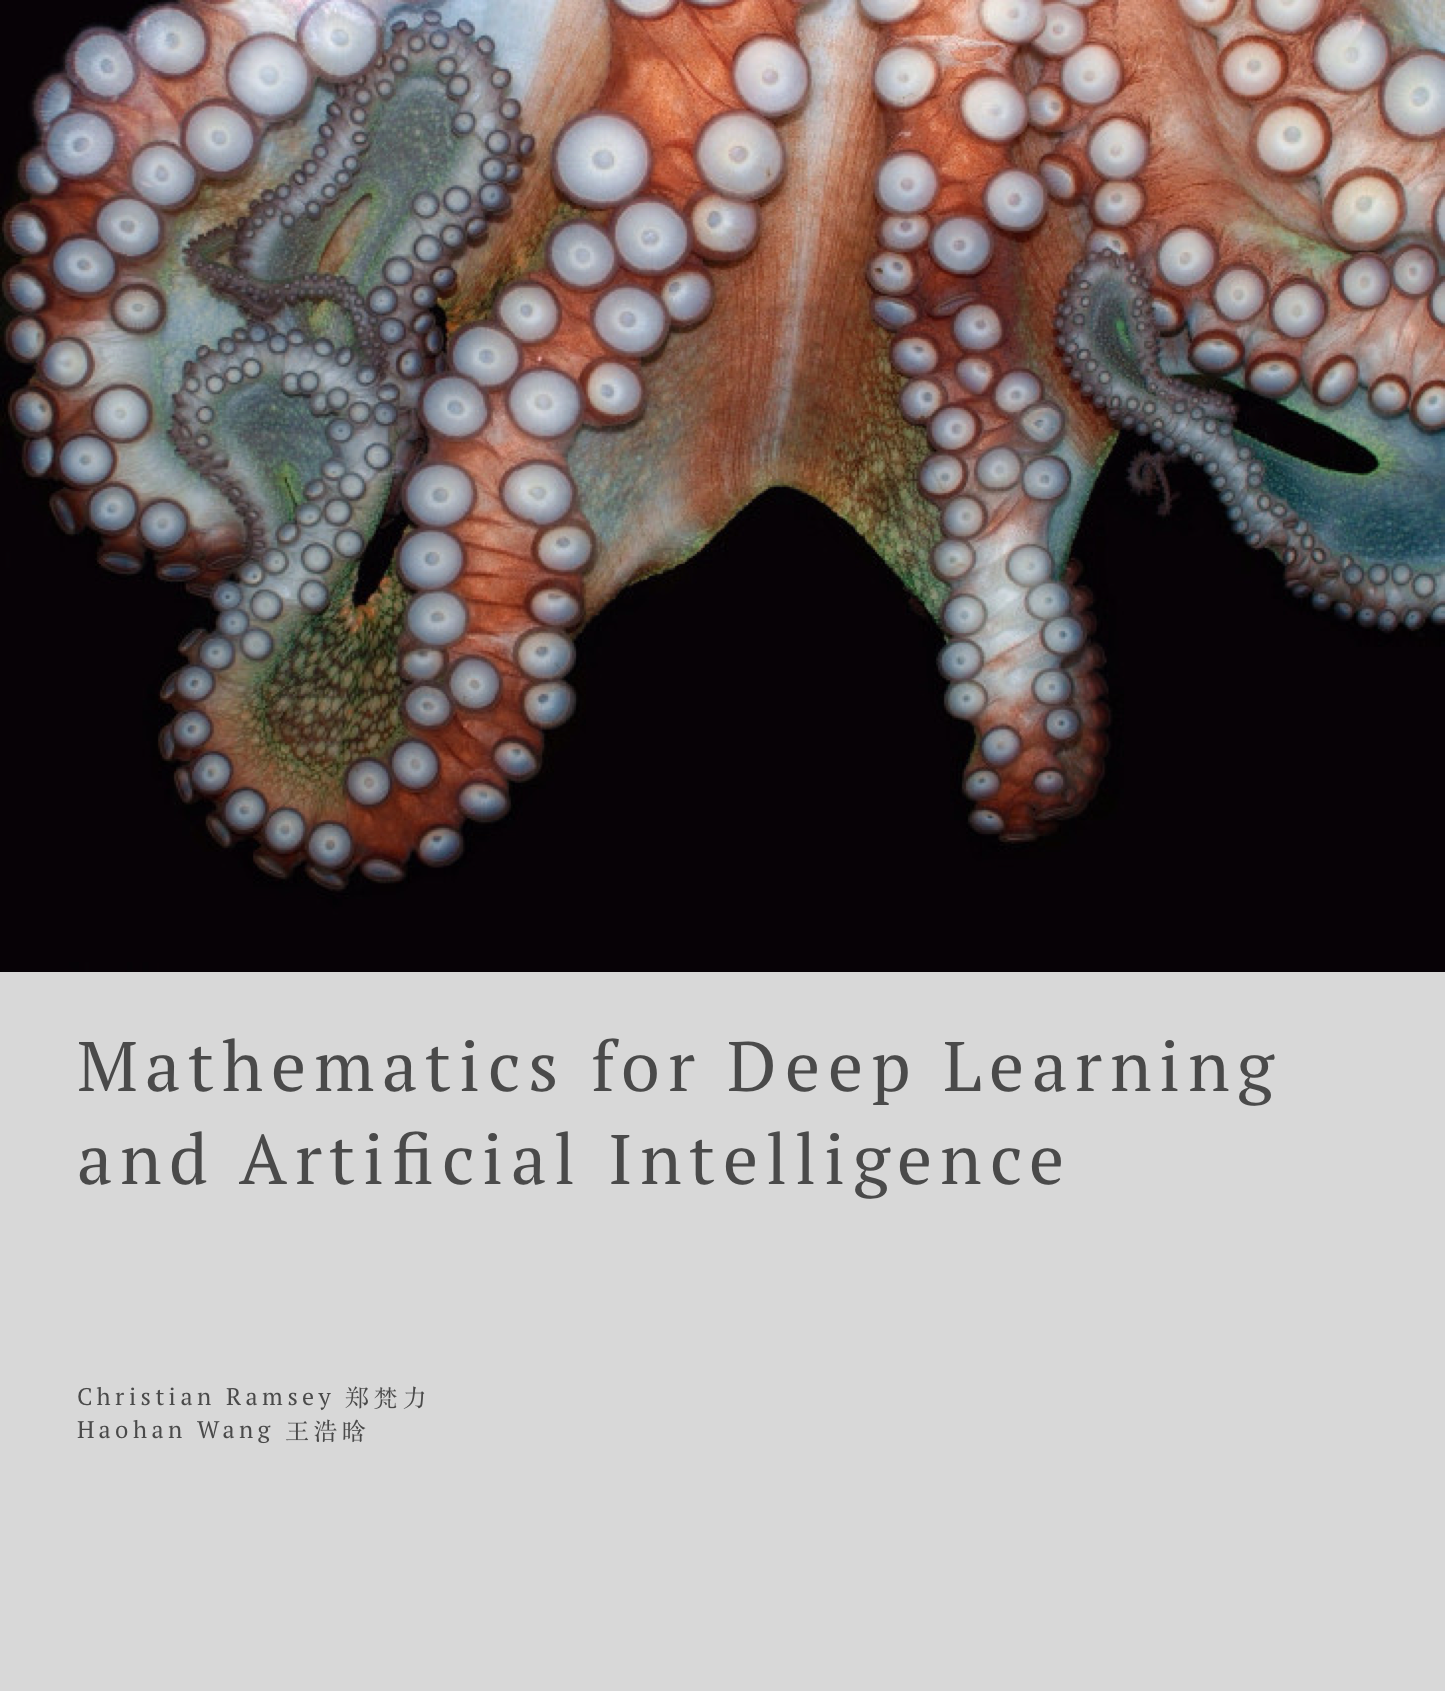
\includegraphics{artwork/maths of deep learning.png}
\caption{Our new book}
\end{figure}

\textbf{Get chapter updates sent to your email.}

\hypertarget{mc_embed_signup}{}
\hypertarget{mc_embed_signup_scroll}{}

\chapter{Introduction to Artificial Intelligence}\label{intro}

..draft.10..

\section{Just what is artificial
intelligence?}\label{just-what-is-artificial-intelligence}

Artificial intelligence is harder to describe in finite terms than it is
to recreate many of the most popular algorithms that serve to represent
it.

\begin{quote}
The definition, if we can say that such a thing exists, is a moving
socio-cultural target and just as we get closer to it's said definition,
it again, slips just outside of our grasp.
\end{quote}

This is partly because AI has always been fundamentally tied up with
some of our deepest philosophical queries and as we make further
progress in AI and related sciences, we again are forced to redraw the
line of what it means to be human.

\begin{quote}
``Nothing that we may know or learn about the functioning of the
organism can give, without `microscopic,' cytological work any clues
regarding the further details of the neural mechanism.'' - Von Neumann
\end{quote}

Generation after generation, we've asked ourselves fundamental questions
that AI, as a philosophical project, touches upon:

\begin{itemize}
\tightlist
\item
  What does it mean to be human?
\item
  What is the difference between humans and other animals?
\item
  Is there another species that is more intelligent than we are
  ++(Übermensch)? +++references
\item
  Will humans be surpassed by a more intelligent species?
\end{itemize}

Neurobiologists like Sapolsky and others, have highlighted that many of
the features we have held so dearly, empathy, politics, culture, tool
usage, are not unique to the human species. It seems that are only true
advantage may be in the sheer number of neurons (86 billion) and
synaptic connections (100 trillion+) between them that has allowed for
more elaborate and subtle ways of those elements unfolding over time.

``We have the same nuts-and-bolts physiology, yet we're using it in very
novel ways. - Robert Sapolsky''

While scientific discoveries continue to redraw the line of what is
truly unique to humans, so does progress in artificial intelligence. So
while it is clear that there is much hype around artificial
intelligence, it can not be argued that there shouldn't be at least some
concern over it's possible futures.

Rather than focus on the takeover, we will focus here on intelligence
and some of the major categorisations that have played a part in today's
AI.

Logic and Reasoning - a type of intelligence that implies the ability of
mental mechanisms to explicitly reason about phenomenon in the world in
a Pattern Recognition/Perception - ++a ty +++what is this?

We will primarily cover the first two subtypes of intelligence in this
book and leave the reader to read more about embodied cognition.

\section{Intelligence as logic and
reasoning}\label{intelligence-as-logic-and-reasoning}

Before we had anything like the first computer, Aristotle and others
were already forming, what we call logic today. Aristotle concerned
himself with what

\begin{itemize}
\tightlist
\item
  what is thinking and reasoning?
\item
  what is it to think and reason well?
\item
  can correct reasoning be mechanized?
\end{itemize}

\begin{quote}
Perhaps there is a logic calculus than can mechanise reasoning
\end{quote}

These are just some of questions that the likes of Aristotle, Leibniz,
Turing, Laplace, Wittgenstein, Gödel, and Boole and others attempted to
answer definitively. Aristotle and the Stoics gave us a framework for
reasoning and propositional logic respectively. Leibniz gave us logical
calculi and a glimpse into computers that could do the same. We also
have George Boole's Boolean algebra (1847) would catch up with Claude
Shannon to begin the digital revolution and progress artificial
intelligence.

Let us think about the context of such questions.

\section{Reasoning and Logic}\label{reasoning-and-logic}

Rene Descartes stated ``Cogito, ergo sum'' which translated means ``I
think therefore I am''. He arrived at this statement after trying to use
pure ``reason'' to find what was fundamentally true without any doubt.
Although he couldn't complete his project, his value of ``reason'' was
not unpopular and is gaining popularity in much of modern culture and
can be heard in everyday conversations when we talk about the
distinction between our thoughts and body.

Reasoning starts with logic.

++Aristotle. +++why is it here

So let us begin with reasoning.

The branch and discipline titled logic was originally focused on finding
absolute truths from statements that could be found in everyday
discourse. Logic is fundamentally tied up with questions around how one
can reason correctly. How one is able to deduce the correct answer given
a set of statements or propositions.

\section{\texorpdfstring{Logic and Biology +++not sure if it is a proper
title I would suggest `From logic to
biology'}{Logic and Biology +++not sure if it is a proper title I would suggest From logic to biology}}\label{logic-and-biology-not-sure-if-it-is-a-proper-title-i-would-suggest-from-logic-to-biology}

\section{Dealing with Uncertainty and
Probability}\label{dealing-with-uncertainty-and-probability}

While Boole was transforming the world of logic, the likes of Komolorov,
Laplace, Jaynes and others were setting out to find a way for us to
better reason when we didn't have complete information and especially
when we had data from several different places.

Jaynes even described probability as an extension of logic. But there
were others who didn't see them as connected at all.

\subsection{Information Theory}\label{information-theory}

While logic and probability were now firmly established, Claude Shannon
combined probability, logic, to create the mathematical theory of
communication which we now call \textbf{Information Theory}.

While probability allows us to reason under uncertainty, Shannon's
information theory allowed us to quantify the uncertainty with a measure
called \(entropy\). This has lead to many concepts including mutual
information, KL divergence, and even a very popular deep learning loss
function. (Encoder-decoder or data compression strategies)

\section{The Rise of AI and
Neuroscience}\label{the-rise-of-ai-and-neuroscience}

\section{Neurobiology and Cognitive
Science}\label{neurobiology-and-cognitive-science}

\subsection{Cortexes}\label{cortexes}

\subsection{Neurons}\label{neurons}

\subsection{Perceptrons and
Perception}\label{perceptrons-and-perception}

The second set of questions were just as philosophically motivated, but
differed in their approaches. Individuals from disciplines like biology,
especially psychology, neurobiology, then called neurophysiology, began
to see that the intelligence of humans and other species may be
uncovered by emulating the central nervous sytem. As we began to
understand an infinitesimally small amount about how a given numnber of
neurons can give rise to intelligent behaviour. ++(Pitts, McCulloch)
give rise to basic intelligence in simpler species like fruitflies to
the advanced intelligence to that of the great apes. +++reference here

Pitts, McCulloch, Rosenblatt, Minsky, and others set out to combine the
advances of logic, from Leibniz's logical calculi to Bool's Boolean
algebra) and combine it with our growing knowledge in brain science
which eventually lead to the creation of the first artificial neural
network, named the perceptron. The first neural network which was based
in the science of logic pushed forward by the likes of Leibniz and
George Boole.

They too had similar questions, ``Can machines think?'', ``Can the brain
be emulated?''. These questions moved away from deductive reasoning and
towards emulating our senses and pereptions. Rosenblatt, Hebb, Minsky,
and others were able to move towards learning from data as humans do by
recognising patterns which birthed ++the first neural network, the
perceptron. +++reference here

This dichotomy, between symbolism and perception, like all dichotomies
don't pin down the reality but we hope that it provides a way of
thinking about our path towards today's artificial intelligence. ++We
are now at a stage where we are bringing what we have learned in
symbolic. +++not sure if I can understand this sentence

\section{The Limits of Logic}\label{the-limits-of-logic}

Though we don't usally think of logic in neural networks, the perceptron
was actually based on logic as you can see from the refrences to Pitts
paper are all around logic.

Godel determined that logic couldn't. Turing found a limit to such
machines. Logic isn't how biological neurons work and limit the capacity
of a neural networks.

\section{Statistical Learning Theory}\label{statistical-learning-theory}

Vapnik, the learnable theorems PAC learning bounds

\section{The modern wave of deep neural
networks}\label{the-modern-wave-of-deep-neural-networks}

Bengio, LeCunn Andrew Ng Hinton, Goodfellow

\section{Deepmind, OpenAI, and so on}\label{deepmind-openai-and-so-on}

\section{Why learn the mathematics of deep
learning}\label{why-learn-the-mathematics-of-deep-learning}

\section{The Mathematics Needed}\label{the-mathematics-needed}

\begin{itemize}
\tightlist
\item
  Logic
\item
  Calculus
\item
  Probability
\item
  Geometry (?)
\item
  Information Theory -- entropy -- mutual information -- bottleneck
\item
  Statistical Learning Theory -- approximation theory -- learnable
\item
  Representation Learning
\item
  Optimization
\end{itemize}

\subsection{Final Thoughts}\label{final-thoughts}

Whatever your motivations for wanting to read the Mathematics of Deep
Learning and Artificial Intelligence, we wish you well on your journey.

++++

++ is the location where I think in question +++ is my comment

Overall I think I like the story and the storyline seems relatively
complete. Somehow the transition from logic to biology is not very well
illustrated. I am expecting to see more explanation about how biology or
even phiolosopy changes the trajector of AI in the last few decades.

You may also need to cover a little bit more about the following
questions:

\begin{itemize}
\tightlist
\item
  what framework of mental model we are following now?
\item
  what is the possible future direction of AI?
\end{itemize}

++++

\chapter{Intro to Logic and
Reasoning}\label{intro-to-logic-and-reasoning}

\section{History of Logic}\label{history-of-logic}

As we all know that Artificial Intelligence (`AI') is the field of
computer science that was developed to enable computers/machines to
display behavior that can be characterized as intelligent.

Then you may ask ``How should we define intelligence? Why are we humans
considered intelligent?''

As I walk you through the history of logic, you will see that our search
for the answer to this question has spanned thousands years. Based on
this journey of `intelligent' search, we can now shed some light on how
and why AI was developed.

As you probably already know humans have long regarded ourselves as
intelligent due to our ability to think and reason.

\begin{quote}
Cogito ergo sum. I think therefore I am - Descartes
\end{quote}

Now, let's begin the journey together to discover one version of the
truth of intelligence.

Logic was developed by
\href{https://en.wikipedia.org/wiki/Aristotle}{Aristotle} (384-322 BCE).
He introduced the formal study of what is now known as `formal logic'.
His logic was concerned with the form, and not the content of statements
or propositions. Basically, Aristotle's system of logic introduced
``hypothetical syllogism'', ``temporal model logic'' and ``inductive
logic''. ** add references to definitions

He claims that a proposition is a complex proposition involving 2 terms,
a subject and a predicate. Each of them are represented with a noun. The
logic form of a proposition is determined by its quantity and it's
quality.

All of Aristotle's logic revolves around one notion: the deduction
(syllogism).

Aristotle says:

\begin{quote}
" A deduction is speech in which, certain things having been supposed,
something different from those supposed results of necessity because of
their being so."
\end{quote}

Each of the `things supposed' is a premise of the argument and what
`results of necessity' is the conclusion.

Following Greek's tradition in logic,
\href{https://en.wikipedia.org/wiki/Cicero}{Cicero} (106-43 BCE)
introduced the term `proposition' for which we will discuss more in
depth later.

\href{https://plato.stanford.edu/entries/alexander-aphrodisias/}{Alexander
of Aphrodisias} (3rd century A.D.) used the term `logic' in the modern
sense of distinguishing correct from incorrect reasoning.

In the early twelfth century,
\href{https://en.wikipedia.org/wiki/Peter_Abelard}{Peter Abelard} wrote
extensive commentaries attempting to articulate issues like opposition,
conversion, quantity, and quality, and composed his treatise, `the
Dialectica'.

Later, \href{https://en.wikipedia.org/wiki/William_of_Sherwood}{William
of Sherwood} developed mnemonic verse as an aid in mastering syllogisms.
Jean Buridan elaborated a theory of consequences which somewhere
??(somewhere) discussed the rules of inference.

Around the same time, Scholastic logician
\href{https://en.wikipedia.org/wiki/Ramon_Llull}{Ramon Llull}, used
logic to prove the Christian faith. He also remarkably designed machines
that would perform logical calculations, and is thus arguably considered
as the father of computer programming. This could be said to have
started the first idea of logic being converted into a machine along
with Charles Babbage's analytical engine.

The traditional logic period starts with
\href{https://en.wikipedia.org/wiki/Antoine_Arnauld}{Antoine Arnauld}
and \href{https://en.wikipedia.org/wiki/Pierre_Nicole}{Pierre Nicole}`s
Logic, or the \emph{Art of Thinking} published in 1662 or the Port Royal
Logic in which logic is defined as the 'art of managing one's reason
right in the knowledge of things, both for the instruction of oneself
and of others'. It was the most influential work on logic in England
until \href{https://en.wikipedia.org/wiki/John_Stuart_Mill}{John Stuart
Mill}'s System of Logic in 1825.

\href{https://en.wikipedia.org/wiki/Gottfried_Wilhelm_Leibniz}{Gottfried
Wilhelm Leibniz} (1646-1716) having invented calculus, concluded that
the whole of logic actually depends on mathematics and thus worked on
reducing scientific and philosophical speculation to computation. He
also suggested that a universal calculus of reasoning could be devised
which would provide an automatic method of solution for all problems
which could be expressed in the universal language. The current
understanding of the power of Leibniz's discoveries did not emerge until
the 1980s.

During the modern and Contemporary Period (1850 - Present), logicians in
the modern period `rediscovered' the Stoic logic of proposition.

People like
\href{https://en.wikipedia.org/wiki/Augustus_De_Morgan}{Augustus De
Morgan} (1806-1864) proposed some ??(some) theorem in that logic which
now bears his name. Considered the founder of symbolic logic and Boolean
Algebra, which is the basis of all modern computer arithmetic.

\href{https://en.wikipedia.org/wiki/George_Boole}{George Boole}
(1815-1864) gave us Boolean Logic which treats propositions as either
true or false. His use of numbers to express the truth values of
compound statements have significantly influenced the development of
computers and he is regarded as being one of the founders of the field
of computer science. Until today, programmers still use his principles
to test the truth of program results or user feedback.

\href{https://en.wikipedia.org/wiki/John_Venn}{John Venn} (1834-1923)
was a Cambridge logician who published 3 standard texts in logic,
\emph{The Logic of Chance 1866}, \emph{symbolic Logic} 1881, and
\emph{The Principles of Empirical Logic} 1889. He is remembered for
introducing the circular diagrams as a tool to test the validity of
syllogisms, known as \textbf{Venn Diagrams}.

Around the same time,
\href{https://en.wikipedia.org/wiki/John_Stuart_Mill}{John Stuart Mill}
(1806-1873) made a thorough study about inductive reasoning and
introduced methods for checking such arguments now known as `Mill's
Methods'. And Charles Sanders Peirce (1839-1914) introduced Pragmatism,
at the core of which he argued that ideas should be evaluated solely by
their practical effects and not by any intrinsic qualities of reason or
logic.\\
** what does this {[}Charles Sanders Peirce{]} mean for the story?

\href{https://en.wikipedia.org/wiki/Gottlob_Frege}{Gottlob Frege}
(1848-1925) pronounced that logic is the basis of mathematics and that
arithmetic and analysis are a part of logic. He has been called the
greatest logician since Aristotle. By developing the \textbf{predicate
calculus} (Quantification Theory), he had combined Aristotelian and
Stoic's logics. His work was the foundation and the beginning point for
an enormous outpouring of work in formal logic.

In 1903, \href{https://en.wikipedia.org/wiki/Bertrand_Russell}{Bertrand
Russell} (1872-1970) started his project `The Principles of Mathematics'
in which he purposed to prove that `all pure mathematics deals
exclusively with concepts definable in terms of a very small number of
logic principles.' Russel also continued the development of the
predicate calculus and he also found the inconsistency in Frege's system
(because Russell's Paradox could be derived within Frege's system).

The next wave of the logic can be called the `mathematical school of
logic'. This tradition or school, includes the work of
\href{https://en.wikipedia.org/wiki/Richard_Dedekind}{Richard Dedekind}
(1831-1916), Giuseppe Peano (1858-1932),
\href{https://en.wikipedia.org/wiki/David_Hilbert}{David Hilbert}
(1862-1943). Ernst Zermelo (1871-1953), and many others since then. Its
goal was the axiomatization of particular branches of mathematics,
including geometry, arithmetic, analysis, and set theory.

In 1889 \href{https://en.wikipedia.org/wiki/Giuseppe_Peano}{Giuseppe
Peano} published the first version of the logical axiomatization of
arithmetic. Five of the nine axioms he came up with are now known as the
Peano axioms. One of these axioms was a formalized statement of the
principle of mathematical induction.

\href{https://en.wikipedia.org/wiki/Ernst_Zermelo}{Ernst Zermelo}'s
axiomatic set theory was also an attempt to escape Russell's Paradox.
His axioms went well beyond Frege's axioms of extensionality and
unlimited set abstraction, and evolved into the now-canonical
Zermelo-Fraenkel set theory.

Gradually, logic became the branch of mathematics that was to be brought
within the axiomatic methodology.
\href{https://en.wikipedia.org/wiki/Jan_\%C5\%81ukasiewicz}{Jan
Łukasiewicz} worked on multi-valued logics. His three-valued
propositional calculus, introduced in 1917, was the first explicitly
axiomatized non-classical logical calculus. ** what does this mean for
logic and AI?

The famous
\href{https://en.wikipedia.org/wiki/Ludwig_Wittgenstein}{Ludwig
Wittgenstein} (1819-1951) entered the list of significant logician by
being one of the developers of the `truth tables'.

This intensive work on mathematical issues culminated in the work of
\href{https://en.wikipedia.org/wiki/Kurt_G\%C3\%B6del}{Kurt Gödel}
(1906-1978), a logician of the caliber of Aristotle and Frege. Using
many applications of the rules of logic, Kurt Godel proved his
`incompleteness theorem', which proposes that some parts of mathematics
are based on ideas that cannot be proved within the system of
mathematics.

Gödel was also one of the central figures in the study of computability.
Others included Alonzo Church (1903-1995), Alan Turing (1912-1954), and
others.

There are plenty of other advances in logic afterwards as well. Logical
empiricist \href{https://en.wikipedia.org/wiki/Rudolf_Carnap}{Rudolf
Carnap} (1891-1970) was associated with the famous verfiability
principle, according to which a synthetic statement is meaninful only if
it is verificable.

Logical positivist \href{https://en.wikipedia.org/wiki/A._J._Ayer}{A.J.
Ayer}, on the other hand, wrote in 1936 his `Language, Truth, and Logic'
in which he focused on the role of language as the medium through which
knowledge is understood and verified.

In 1965, \href{https://en.wikipedia.org/wiki/Lotfi_A._Zadeh}{Lotfi A.
Zadeh} developed `fuzzy logic' which allows imprecise answers to
questions in addition to being either clear-cut true or false. This
logic now serves as the basis of computer programming designed to mimic
human intelligence.

Let's pause here for a while and take a close look at the progress that
made by Alan Turing,
\href{https://en.wikipedia.org/wiki/Alonzo_Church}{Alonzo Church} and
Kurt Godel during this period.

As we all know that,
\href{https://en.wikipedia.org/wiki/Alan_Turing}{Alan Turing}, the
father of computing, created a machine that can accept different
instructions for different tasks in 1936 and marked the first step of
the AI with his seminal 1950 paper. Turing's initial investigation of
computation stemmed from the programme set out by David Hilbert in 1928.
Hibert presented 3 open questions for logic and mathematics. Was
mathematics \ldots{}

\begin{enumerate}
\def\labelenumi{\arabic{enumi}.}
\item
  \emph{complete} in a sense that any mathematical assertion could
  either be proved or disproval
\item
  \emph{consistent} in the sense that false statements could not be
  derived by a sequence of valid steps and
\item
  \emph{decidable} in the sense that there exists a definite method to
  decide the truth of falsity of every mathematical assertion.
\end{enumerate}

Within 3 years, Kurt Godel had proved that the axioms of arithmetic are
both not complete and consistent. By 1937 both Alonzo Church and Alan
Turing had demonstrated that undecidability of particular mathematical
assertions. Interestingly, as Godel and Church had depended on
demonstrating their results using purely mathematical calculi. Turing
chose to take an unusual route of considering mathematical proof as an
artifact of human reasoning. He even generalized this notion to a
physical machine that he believes it could emulate a human mathematician
and in turn there could be a universal machine that can emulate all
other computing machines. Then he used this construct to show that
certain functions cannot be computed by such a universal machine and in
turn, demonstrated the undecidability of assertions associated with such
functions.

As we can easily tell, at the heart of Turing's universal machine is a
model of human reasoning and calculation. After putting his idea into
practice during the World War II, he came up with a comprehensive paper
that provided a philosophical framework for answering the question `Can
machines think?' i.e.~the invention of the `Turing test' and
universality of digital computers. He also goes on to discuss 2 distinct
strategies that might be considered possible of achieving a thinking
machine:

\begin{quote}
AI by programming
\end{quote}

\begin{quote}
AI by machine learning
\end{quote}

\begin{quote}
AI using logic, probabilities, learning and background knowledge
\end{quote}

As you can see from history, the endeavors of implementing these
strategies have been carrying on simulatenously in the last few decades.
Here let's just take a close look at the last proposed approach \emph{AI
using logic, probabilities, learning and background knowledge}.

\begin{quote}
``It is necessary there to have some other `unemotional' channels of
communication. If there are available it is possible to teach a machine
by punishments and rewards to obey orders given in some language, e.g.~a
symbolic language. There orders are to be transmitted through the
`unemotional' channels. The use of this language will diminish greatly
the number of punishment and reward required.'' - Alan Turing
\end{quote}

As for how to achieve it, he said:

\begin{quote}
``Opinions may vary as to the complexity which is suitable in the child
machine. One might try to make it as simple as possible, consistent with
the general principles. Alternatively, one might have a complete system
of logical inference `built in'. In the latter case, the store would be
largely occupied with definitions and propositions.''
\end{quote}

**chain the above paragraph with the one below by relation

Here are some attempts that we have made after Turing's proposal. After
the introduction of resolution-based automatic theorem introduced by
Alan Robinson in 1965. The interest of using first-order predicate
calculus as a representation for reasoning within AI systems
skyrocketed. Also, as introduced in Gordon Plotkin's thesis, it became
possible for us to use resolution theorem proving to investigate a form
of machine learning that involves hypothesising logical axioms from
observations to background knowledge.

Now let's go back to our initial question about AI. As we can see from
the above journey, AI has been heavily influenced by some of these
logical ideas. Undoubtedly, logic has played an crucial role in some
central areas of AI research. As much as we are trying to compute our
reasoning process, the ultimate goal of a thinking machine is to be able
to formalize \emph{common} \emph{sense} \emph{reasoning}, the
prescientific reasoning that is used in handling everyday problems.

In order to take on this mission, we just created a whole new set of
problems for ourselves to deal with i.e.~knowledge representation and
reasoning for which we will discuss more in depth in the later chapter.
In short, inspired by psychology and neurobiology about how we humans
solve problems and represent knowlege of the world.

Talking about the connection of AI, logic and neurophysiology, we have
brought up these 2 men,
\href{https://en.wikipedia.org/wiki/Warren_Sturgis_McCulloch}{Warren
Sturgis McCulloch} and
\href{https://en.wikipedia.org/wiki/Walter_Pitts}{Walter Pitts}.
McCulloch was a psychologist, psychiatrist and philosopher by degree,
but he had been working on and thinking about how to apply
neurophysiology and logic to model the brain. Upon the time he met
Pitts, a homeless young man who had been hanging around the University
of Chicago, they realized that they shared a same hero in common:
Gottfried Leibniz. As what have mentioned before, Leibniz is the
inventor of calculus and he also had attempted to create a computing
system that can replicate human thoughts, in which each letter
represented a concept and they could be combined and manipulated
according to a set of logical rules. As a numerous logicians and
philosophers had tried, it is an attempt and a vision that promised to
transform the chaotic outside world into the rational and organized
system.

In their paper
\href{http://www.cs.cmu.edu/~epxing/Class/10715/reading/McCulloch.and.Pitts.pdf}{A
Logical Calculus of Ideas Immanent in Nervous Activity}, they introduced
the idea of artificial neural network. This had been inspired by
Leibnizian logical calculus and
\href{https://en.wikipedia.org/wiki/Principia_Mathematica}{Principia
Mathematica}, they created a network that uses logical predicate to
compute as they were convinced that the brain was just such a machine
that uses logic encoded in neural networks to compute.

As you probably have had predicted, these two men started to work on
this idea of capturing reasoning with a logical calculus. But this time,
they also tried a novel approach which is to combine the knowledge of
biological neurons. By stringing the simple neurons into chains and
loops, they had shown that it is possible for brain to implement every
possible logical operation and outputting anything that could be
calculated by one of Turing's hypothetical machines.

As what they put:``Because of the `all-or-none' character of nervous
activity, neural events and the relations among them can be treated by
means of propositional logic.'', they divided neurons into 2 groups,
*peripheral afferents (or `input neurons') and the rest ('output
neurons) and each neuron can be in 2 states, firing or non-firing. They
defined every neuron i a predicate which is true when the neuron is
firing at the moment t. As for the solution of this network,
\(N_i(t) \equiv B\) here B is a conjunction of firings from the previous
moment of the peripheral afferents, and i is not an input neurons. It is
also worth to mention that this paper has only three references, and all
of them are classical works in logic:

\begin{itemize}
\item
  Carnap, R. 1938.
  \href{https://archive.org/details/in.ernet.dli.2015.136409/page/n5}{The
  Logical Syntax of Language}. New York: Harcourt-Brace.
\item
  Hilbert, D. and W. Ackermann. 1927.
  \href{https://www.springer.com/us/book/9783642654015}{Grundzüge der
  Theoretischen Logik}. Berlin: Springer.
\item
  Russell, B. and A. N. Whitehead. 1925.
  \href{https://en.wikipedia.org/wiki/The_Principles_of_Mathematics}{Principa
  Mathematics}. Cambridge University Press.
\end{itemize}

Here is also a longer version of the story of Pitts and Mccolloch that I
won't cover here. In short, there are plenty of other brilliant minds
like Jerome Lettvin, Norbert Weiner, von Neumann have contributed to the
invention of cybernetics. You can think of the story of Pitts and
McCulloch is also the story of cybernetics which was born out of the
influences of ideas from a variety of domains and fields, and in a way a
neural network symbolizes this interaction.

If you are interested in knowing more about the cybernetics and the
story of McColloch and Pitts Walter, don't forget to check this article
out:
\href{http://nautil.us/issue/21/information/the-man-who-tried-to-redeem-the-world-with-logic}{The
Man Who Tried to Redeem the World with Logic}.

After the age of Pitts and McColloch, there were 2 major trens
underlying the research in Artificial Intelligence around 1960s. The
first trend produced thre program that uses symbolic reasoning/deducive
logical systems. People like
\href{https://en.wikipedia.org/wiki/Herbert_A._Simon}{Herbert A. Simon},
\href{https://en.wikipedia.org/wiki/Allen_Newell}{Allen Newell} and
\href{https://en.wikipedia.org/wiki/Cliff_Shaw}{Cliff Shaw} have created
some working programs based on this principles. The reason the symbolic
systems are somewhat appealing is that they seemed to be able to provide
the control and extensibility that neural network could not. Due to the
function that symbolic systems have achieved i.e.~proving theorems and
playing chess, we would conclude that

\begin{quote}
symbolic thinking is considered a rare and desirable aspect of
intelligence in humans, but it comes rather natural to computers which
have much more trouble with reproducing 'low-level'intelligent behavior
that comes very natural to human, such as recognizing the animal in the
picture and picking up objects.
\end{quote}

This is the famous Moravec's Paradox discovered by
\href{https://en.wikipedia.org/wiki/Hans_Moravec}{Hans Moravec} in
1980s. You can simplify the statement as \textbf{``Robots find the
difficult things easy and the easy things difficult.''}

All those discoveries helped us to begin doubting about our initial
belief ``we think therefore we are''. Brought us back to our initial
profound philosophical question:``what makes us human intellient?''

Again, we stumble upon the crux of the issue - most of the intellectual
and scientific discipline of modernity are ultimately premised upon
philosophical assumptions. As much as we hate to admit the possible
limit of AI, we may need to revisit this question with a new framework
or mental model. As philosophier
\href{https://en.wikipedia.org/wiki/Hubert_Dreyfus}{Hubert Dreyfus}
suggested, drawing from the work of
\href{https://en.wikipedia.org/wiki/Martin_Heidegger}{Martin Heidegger}
and \href{https://en.wikipedia.org/wiki/Maurice_Merleau-Ponty}{Maurice
Merleau-Ponty} the brain does not create internal representations of
objects in the world. The brain simply learns how to see the world
directly. Or as Rodney Brooks said:``the best model for the world is the
world itself.'' In constrast to the classic AI `computational theory of
mind', the embodied robot will continuously refer to its sensors rather
than to an internal world model/representation just as we humans do.

Though it seems true that the `thinking machine' cannot be built with
logic solely, logic in AI currently is still a large and rapidly growing
field. One of the most influential figure in logical AI is John
McCarthy. McCarthy was also one of the founders of AI, and consistently
advocated a research methodology that uses logical techniques to
formalize the reasoning problems that AI needs to solve. You may wonder,
what motivates them to continue integrating logic with AI. The answer is
that a logical formalization helps us to understand the reasoning
problem itself. However, as we currently know, the key to solve a
problem may not need an thorough understanding of what the reasoning
problems are. It is in fact quite controversial in the context of AI, an
alternative methodology would be for such a machine to learn or evolve
the desired behaviors.

\subsection{The End of Logic?}\label{the-end-of-logic}

The intellectual project to capture thinking in terms of logic was at
first thought to solve the problem of reasoning only to find out later
that what makes human intelligent isn't just reasoning, but reasoning
under uncertain conditions as well as learning not just from rules but
from the world itself.

So it is not the end of logic, for it powers so much of modern
computing, but like any grand theory that takes on something as complex
as human level thinking it has found it's practical place as a tool
forever in our intellectual and computational toolbelt.

I would like to leave you with this last provoking statement from
Longuet-Higgins:``We need AI not to build machines, but to understand
humans.''

**this is really amazing and thorough. I like the way the second half
reads better than the first because it's less of a reading of the facts.
It would be great if you could relate the discovering together and their
relation to AI. As a next step, I would leave this how it is with my
corrections and then write a second one that is half as long and a kid
could read. Great job.

\bibliography{book.bib,packages.bib}


\end{document}
